\chapter{High Energy QCD}
\label{chap:HEQCD}

\section{The High Energy Limit of $2\rightarrow2$ QCD scattering}

	\subsection{Quark-Gluon scattering at High Energy}

		We start with the simplest case of $2\rightarrow 2$ quark-gluon scattering which consists of three
		diagrams shown in figure \ref{fig:TwoToTwo}.  Here we only show the calculations for the helicity
		structure where both quarklines have fixed, and opposite, helicities.  We use the following gauge
		choice for the gluon polarisations:

		\begin{align}
		\epsilon^{+*}_{2\sigma}&=\frac{\langle b|\sigma|2\rangle}{\sqrt{2}\langle b2\rangle} & \epsilon^{-*}_{2\sigma} &= -\frac{\langle b|\sigma|2\rangle}{\sqrt{2}[b2]} \\
		\epsilon^{+}_{b\sigma}&=-\frac{\langle b|\sigma|2\rangle}{\sqrt{2}[2b]} & \epsilon^{-*}_{2\sigma} &= -\frac{\langle b|\sigma|2\rangle}{\sqrt{2}\langle 2b\rangle}
		\end{align}

		For simplicity we alter the notation slightly and choose to model everything as having negative helicity.  To describe positive helicities we can use the transpose property shown in equation 16.

		% \begin{figure}
		% \begin{center}
		% \includegraphics[width=0.9\linewidth]{TwoToTwo.eps}
		% \caption{Feynman diagrams showing the $qg\rightarrow qg$ processes at tree level.}
		% \label{fig:TwoToTwo}
		% \end{center}
		% \end{figure}

		\subsubsection{$s$-channel}

			The matrix element for the $s$-diagram is:

			\begin{equation}
			-i\mathcal{A}_s=\overline{u}^-(p_1)\left(-\frac{ig_s}{2}\gamma^\mu\right)\epsilon_\mu^{*+}(p_2)\frac{i(\slashed q+mc)}{q^2-m^2c^2}\left(-\frac{ig_s}{2}\gamma^\nu\right)\epsilon^+_\nu(p_b)u^-(p_a),
			\end{equation}
			\begin{equation*}
			\Rightarrow \mathcal{A}_s=-\frac{g^2_s}{4q^2}\epsilon^{*+}_{2\mu}\epsilon^+_{b\nu}\overline{u}^-_1\gamma^\mu\slashed q\gamma^\nu u^-_a,
			\end{equation*}

			where we have used $q\gg mc$ for the high energy case.  The propagator has momentum $q=p_a+p_b=p_1+p_2$ therefore:

			\begin{equation}
			\mathcal{A}_s=-\frac{g^2_s}{4q^2}\frac{\langle{b}|\mu|2\rangle}{\sqrt{2}\langle{b2\rangle}}\frac{\langle{b}|\nu|2\rangle}{\sqrt{2}[2b]}\overline{u}^-_1\gamma^\mu(\slashed{p}_a+\slashed{p}_b)\gamma^\nu u^-_a,
			\end{equation}
			\begin{equation*}
			\Rightarrow\mathcal{A}_s=-\frac{g^2_s}{8q^2s_{2b}}\langle{b}|\mu|2\rangle\langle{b}|\nu|2\rangle\left(\overline{u}^-_1\gamma^\mu\gamma^\sigma\gamma^\nu u^-_ap_{a\sigma}+\overline{u}^-_1\gamma^\mu\gamma^\sigma\gamma^\nu u^-_ap_{b\sigma}\right),
			\end{equation*}

			where we have used equation 8.  The gamma matrices satisfy the Clifford algebra, $\{\gamma^\mu, \gamma^\nu\}=2g^{\mu\nu}$ and so we may write:

			\begin{equation}
			\overline{u}^-_1\gamma^\mu\gamma^\sigma\gamma^\nu u^-_ap_{a\sigma}=\overline{u}^-_1\gamma^\mu\gamma^\nu\gamma^\sigma u^-_ap_{a\sigma} - 2\overline{u}^-_1\gamma^\mu g^{\sigma\nu}u^-_ap_{a\sigma}
			\end{equation}

			But in the MRK limit the Dirac equation is $\slashed{p}_au^-_a=0$:

			\begin{equation}
			\mathcal{A}_s=-\frac{g^2_s}{8q^2s_{2b}}\langle{b}|\mu|2\rangle\langle{b}|\nu|2\rangle\left(-2\overline{u}^-_1\gamma^\mu u^-_ap_{a}^\sigma+\overline{u}^-_1\gamma^\mu\gamma^\sigma\gamma^\nu u^-_ap_{b\sigma}\right)
			\end{equation}

			For the second term we must use the following identity:

			\begin{equation}
			\gamma^\mu\gamma^\sigma\gamma^\mu=g^{\mu\sigma}\gamma^\nu + g^{\sigma\nu}\gamma^\mu - g^{\mu\nu}\gamma^\sigma - i\epsilon^{\rho\mu\sigma\nu}\gamma_\rho\gamma^5,
			\end{equation}

			where $\epsilon^{\rho\mu\sigma\nu}$ is the $4D$ totally antisymmetric symbol:

			\begin{equation}
			\mathcal{A}_s=-\frac{g^2_s}{8q^2s_{2b}}\langle{b}|\mu|2\rangle\langle{b}|\nu|2\rangle
			\left(\langle 1|\mu|a\rangle p_a^\nu + p_{b\sigma}\overline{u}^-_1(g^{\mu\sigma}\gamma^\nu + g^{\sigma\nu}\gamma^\mu - g^{\mu\nu}\gamma^\sigma - i\epsilon^{\rho\mu\sigma\nu}\gamma_\rho\gamma^5)\right)
			\end{equation}
			\begin{equation}
			\Rightarrow\mathcal{A}_s=-\frac{g^2_s}{8q^2s_{2b}}\langle{b}|\mu|2\rangle\langle{b}|\nu|2\rangle
			\left(\langle 1|\mu|a\rangle \langle a|\nu|a\rangle\!+\!\langle b|\mu|b\rangle\langle 1|\nu|a\rangle\!+\!\langle b|\sigma|b\rangle\langle1|\sigma|a\rangle
			g^{\mu\nu}\!-\!i\langle b|\sigma|b\rangle\langle 1|\epsilon^{\rho\mu\sigma\nu}\gamma_\rho\gamma^5|a\rangle\right)
			\end{equation}

			The second, third and fourth terms are zero because, for example:

			\begin{equation}
			\langle b|\mu|2\rangle\langle b|\mu|b\rangle = 2[2b]\langle b b\rangle = 0
			\end{equation}

			\begin{equation}
			\Rightarrow\mathcal{A}_s=-\frac{g^2_s}{8q^2s_{2b}}\langle{b}|\mu|2\rangle\langle{b}|\nu|2\rangle\langle{1}|\mu|a\rangle\langle{a}|\nu|a\rangle
			\end{equation}

			Where we have used equation 10.

			\begin{equation}
			\mathcal{A}_s=-\frac{g^2_s}{4q^2s_{2b}}[2a]\langle ab\rangle\langle{b}|\mu|2\rangle\langle{1}|\mu|a\rangle
			\end{equation}

			And using $q^2=s_{ab}=\langle ab\rangle[ba]$ and $s_{2b}=\langle2b\rangle[b2]$ we have:

			\begin{equation}
			\mathcal{A}_s=-\frac{g^2_s}{4}\frac{[2a]\langle ab\rangle}{\langle ab\rangle[ba]\langle2b\rangle[b2]}\langle{b}|\mu|2\rangle\langle{1}|\mu|a\rangle.
			\end{equation}

			Now all that remains is to calculate the four-vector products, for example:

			\begin{equation}
			[2a]=\overline{u}^+_2u^-_a=(u^+_2)^\dagger\gamma^0u^-_a=\left(\sqrt{p^+_2}, \sqrt{p^-_2}\frac{p^{\perp}_2}{|p_2^\perp|}, 0, 0\right) \left(\begin {array}{cccc} 0&0&1&0\\ \noalign{\medskip}0&0&0&1
			\\ \noalign{\medskip}1&0&0&0\\ \noalign{\medskip}0&1&0&0\end {array}\right)\left( \begin {array}{c} 0\\ \noalign{\medskip}0\\ \noalign{\medskip}0\\ \noalign{\medskip}-\sqrt{p^+_a}\end {array}\right)
			\end{equation}
			\begin{equation}
			[2a]=\left(\sqrt{p^+_2}, \sqrt{p^-_2}\frac{p^{\perp}_2}{|p_2^\perp|}, 0, 0\right)\left( \begin {array}{c} 0\\ \noalign{\medskip}-\sqrt{p^+_a}\\
			\noalign{\medskip}0\\ \noalign{\medskip}0\end {array}\right)=-\frac{\sqrt{p_a^+p_2^-}p_2^\perp}{|p_2^\perp|}
			\end{equation}

			And similarly for the others yielding:

			\begin{equation}
			\mathcal{A}_s=-\frac{g_s^2}{4}\sqrt{\frac{p_2^-}{p_b^-}}\frac{1}{p_2^+p_b^-}\frac{p_2^{\perp^*}}{|p_2^\perp|}\langle{b}|\mu|2\rangle\langle{1}|\mu|a\rangle
			\end{equation}

			Which can be simplified slightly since $\hat{t}=s_{2b}$ to give the final result:

			\begin{equation}
			\mathcal{A}_s=-\frac{g_s^2}{2\hat{t}}\sqrt{\frac{p_2^-}{p_b^-}}\frac{p_2^{\perp^*}}{|p_2^\perp|}\langle{b}|\mu|2\rangle\langle{1}|\mu|a\rangle
			\end{equation}

		\subsubsection{$t$-channel}

		The matrix element for the $t$-diagram is:

			\begin{equation}
			\begin{split}
			-i\mathcal{A}_t &=-\overline{u}^-_1\left(-\frac{ig_s}{2}\gamma^\mu\right)\left(-\frac{ig_{\mu\nu}}{q^2}\right)u^-_ag_sf^{\gamma\beta\delta}
			\left(g_{\sigma\nu}(p_b-q)_\rho + g_{\nu\rho}(p_b-q)_\sigma - g_{\rho\sigma}(p_b-q)_\nu)\right)\epsilon^{\rho *}_{2+}\epsilon^{\sigma}_{b+}\\
			i\mathcal{A}_t &=-\frac{g_s^2}{2q^2s_{2b}}\left(\overline{u}^-_1\gamma^{\nu}u^-_a\right)\left(\overline{u}^-_b\gamma^{\rho}u^-_2\right)
			\left(\overline{u}^-_b\gamma^{\sigma}u^-_2\right)\left(g_{\sigma\nu}(p_b-q)_\rho + g_{\nu\rho}(p_b-q)_\sigma - g_{\rho\sigma}(p_b-q)_\nu)\right)
			\end{split}
			\end{equation}

			Now using $q=p_a-p_1=p_2-p_b$:

			\begin{align*}
			i\mathcal{A}_t = -\frac{g_s^2}{2q^2s_{2b}}&[(2p_{2\rho}-p_{b\rho})\left(\overline{u}^-_1\gamma_{\sigma}u^-_a\right)\left(\overline{u}^-_b\gamma^{\rho}u^-_2\right)\left(\overline{u}^-_b\gamma^{\sigma}u^-_2\right)+\ldots \\
			\ldots +&\hspace{2pt} (2p_{2\sigma}-p_{b\sigma})\left(\overline{u}^-_1\gamma_{\nu}u^-_a\right)\left(\overline{u}^-_b\gamma^{\nu}u^-_2\right)\left(\overline{u}^-_b\gamma^{\sigma}u^-_2\right)-\ldots \\
			\ldots -&\hspace{2pt} (p_{2\nu}\hspace{4pt}+p_{b\nu})\left(\overline{u}^-_1\gamma^{\nu}u^-_a\right)\left(\overline{u}^-_b\gamma_{\sigma}u^-_2\right)\left(\overline{u}^-_b\gamma^{\sigma}u^-_2\right)]
			\end{align*}

			Once again in the high energy case the Dirac equation is $\slashed pu^\pm=0$ and $\overline{u}^\pm\slashed p=0$.  The first line of the above expression reads:

			\begin{equation}
			2\langle1|\sigma|a\rangle\langle b|\sigma|2\rangle\overline{u}^-_b\slashed p_2u^-_2 - \langle1|\sigma|a\rangle\langle b|\sigma|2\rangle\overline{u}^-_b\slashed p_b,
			\end{equation}

			which is clearly zero.  The other two lines contain similar factors and therefore $\mathcal{A}_t=0$.
			This seems strange since we want to show that the $t$-channel dominates!  It is \emph{only} in this
			gauge that $\mathcal{A}_t$ vanishes as the gauge effectively just shuffles the contributions to the
			sum between the channels.

		\subsubsection{$u$-channel}

		The matrix element for the $u$-diagram is:

			\begin{equation}
			\begin{split}
			-i\mathcal{A}_u &= \overline{u}^-(p_1)\left(-\frac{ig_s}{2}\gamma^\mu\right)\frac{i(\slashed q+mc)}{q^2-m^2c^2}\left(-\frac{ig_s}{2}\gamma^\nu\right)u^-(p_a)\epsilon_\mu^{*+}(p_b)\epsilon^+_\nu(p_2)\\
			\mathcal{A}_u &= \frac{g_s^2}{4q^2}\overline{u}^-_1\gamma^\mu\slashed q\gamma^\nu u^-_a\epsilon^{+*}_{b\mu}\epsilon^*_{2\nu}\\
			&= \frac{g_s^2}{8q^2s_{2b}}\langle b|\mu|2\rangle\langle b|\nu|1\rangle\overline{u}^-_1\gamma^\mu(\slashed{p}_a-\slashed{p}_2)\gamma^\nu u^-_a\\
			&= \frac{g_s^2}{8q^2s_{2b}}\langle b|\mu|2\rangle\langle b|\nu|1\rangle(\overline{u}^-_1\gamma^\mu\gamma^\sigma\gamma^\nu u^-_ap_{a\sigma} - \overline{u}^-_1\gamma^\mu\gamma^\sigma \gamma^\nu u^-_ap_{2\sigma})
			\end{split}
			\end{equation}

			Where we have used $q=p_a-p_2$.  By direct comparison with the procedure used for the $s$-channel we can see the result will be:

			\begin{equation}
			\mathcal{A}_u=\frac{g_s^2}{2\hat{t}}\sqrt{\frac{p_b^-}{p_2^-}}\frac{p_2^{\perp^*}}{|p_2^\perp|}\langle{b}|\mu|2\rangle\langle{1}|\mu|a\rangle.
			\end{equation}

			The \emph{total} total matrix element is therefore:

			\begin{equation}
			\mathcal{A}=\frac{g_s^2}{2}\frac{p_2^{\perp^*}}{|p_2^\perp|}\left(\sqrt{\frac{p_b^-}{p_2^-}}-\sqrt{\frac{p_2^-}{p_b^-}}\right)\frac{\langle{b}|\mu|2\rangle\langle{1}|\mu|a\rangle}{\hat{t}},
			\label{eqn:fullsum}
			\end{equation}

			Which is exactly in the currents form i.e. in the form $\frac{j_a^\mu\cdot j_{b_\mu}}{\hat{t}}$.  In the MRK
			limit we have $p_b^-\thicksim p_2^-$ and so equation \ref{eqn:fullsum} can be simplified further (we actually
			choose \emph{not} to take this option so as to include as few approximations as possible).  The important
			thing about equation 41 is that this helicity structure can be described exactly at the MRK limit by the
			exchange of a soft $t$-channel gluon.  Although all of the other valid helicity combinations must be
			calculated too we see they also have a $\hat t$ pole.

	\subsection{Mandelstam Variables in the High Energy Limit}
	\label{sub:Mandelstam Variables in the High Energy Limit}

		The $2\rightarrow 2$ QCD scattering amplitudes can be expressed in terms of the well-known Mandestam variables $s$, $t$ and $u$.  Which, in terms of the momenta in the process, are given by:

		\begin{subequations}
			\begin{equation}
				s = (p_1 + p_2)^2
			\end{equation}
			\begin{equation}
				t = (p_1 - p_2)^2
			\end{equation}
			\begin{equation}
				u = (p_2 - p_3)^3
			\end{equation}
		\end{subequations}

		When working in the high energy limit it is convenient to re-express these in terms of the perpendicular momentum of the outgoing partons, $p_\perp$, and the difference in rapidity between the two final state partons, $\delta y$:

		\begin{subequations}
			\begin{equation}
				s = 4p_\perp^2 \cosh^2\frac{\Delta y}{2}
			\end{equation}
			\begin{equation}
				t = -2p_\perp^2 \cosh\frac{\Delta y}{2}e^{-\frac{\Delta y}{2}}
			\end{equation}
			\begin{equation}
				u = -2p_\perp^2 \cosh\frac{\Delta y}{2}e^{\frac{\Delta y}{2}}
			\end{equation}
		\end{subequations}

		In the limit of hard jets well separated in rapidity these can be approximated to give

		\begin{subequations}
			\begin{equation}
				s \approx p_\perp^2 e^{\Delta y}
			\end{equation}
			\begin{equation}
				t \approx -p_\perp^2
			\end{equation}
			\begin{equation}
				u \approx -p_\perp^2 e^{\Delta y}
			\end{equation}
		\end{subequations}

		From eq. (above) it is clear that the `hard, wide-angle jet' limit is equivalent to the High Energy limit since:

		\begin{equation}
			\Delta y \approx \ln \left(\frac{s}{-t}\right)
		\end{equation}

	\subsection{HE limit of the three-gluon vertex}
	\label{sub:subsection_name}

		The three gluon vertex shown in fig. (X) has the following Feynman rule:

		\begin{equation}
			g_s f^{abc} \left((p_1+p_3)^\nu g^{\mu_1\mu_3} + (q-p_3)^{\mu_1}g^{\mu_3\nu} - (q+p_1)^{\mu_3}g^{\mu_1\nu}\right)
		\end{equation}

		In the high energy limit the emitted gluon with momenta $q$ is much softer that the emitting gluon with momenta $p_1$ i.e. $p_1^\mu \gg q^\mu$  $\forall \mu$ and therefore $p_1\sim p_3$ - using this we can approximate the vertex by

		\begin{equation}
			\approx g_s f^{abc} \left(2p_1^\nu g^{\mu_1\mu_3} + p_3^{\mu_1}g^{\mu_3\nu} - p_3^{\mu_3}g^{\mu_1\nu}\right)
		\end{equation}

		Furthermore, since the hard gluons in a high energy process are external they must satisfy the Ward identities; $\epsilon_1\cdot p_1 = \epsilon_3\cdot p_3 = 0$.  Hence, the vertex can be expressed simply as:

		\begin{equation}
			\approx 2g_s f^{abc}p_1^\nu g^{\mu_1\mu_3}
		\end{equation}

	\subsection{At Leading Order in $\alpha_s$}
	\label{sub:HE22_LO}

		Talk through the limit of $2\rightarrow2$ scattering of gluons.  Introduce mandelstam variables, show the equivalence of large delta y and large s.

	\subsection{At Next-to-Leading Order in $\alpha_s$}
	\label{sub:HE22_NLO}

		Calculate the NLO calcuations to the 2j ME and show that there explicitly is a delta y (large log) enhancement.

	\subsection{High Energy Jets `Currents'}
	\label{sub:currents}

	\subsection{Effective Vertices For Real Emissions}
	\label{sub:effective_vertices_for_real_emissions}

\section{High Energy Jets}
\label{sec:section_name}

	\subsection{The Multi-Regge Kinematic limit of QCD amplitudes}
	\label{sub:subsection_name}

	\subsection{Logarithms in HEJ observables}
	\label{sub:subsection_name}

		Here you should take a $2\rightarrow n$ ME, apply the HE limit to it, do a PS integration and show the logs you get.  Need the HE limit of PS integral from JA thesis and/or from VDD talk

	\subsection{HEJ currents}
	\label{sub:currents}

	\subsection{High Energy Phase-space Integration}
	\label{sub:HEPhaseSpace}

